\chapter{Frameworks para ETL}

\noindent Este capítulo apresenta os principais \textit{frameworks} correlatos a este trabalho encontrados na literatura, bem como os descreve  demonstrando suas características, seus pontos positivos e negativos.
\clearpage



\section{ARKTOS II}

O principal objetivo do ARKTOS II é facilitar a modelagem dos processos de ETL, de forma que o usuário define a fonte dos dados e o destino, os participantes e o fluxo de dados do processo. Como ilustrado na figura \ref{arktosii}, o usuário pode desenhar atributos e parâmetros, conectá-los ao seu esquema de dados, criar relacionamentos e desenhar arestas de um nó para outro de acordo com a arquitetura do grafo (\cite{vassiliadis:2005}).


\begin{figure}[h]
	\centering
	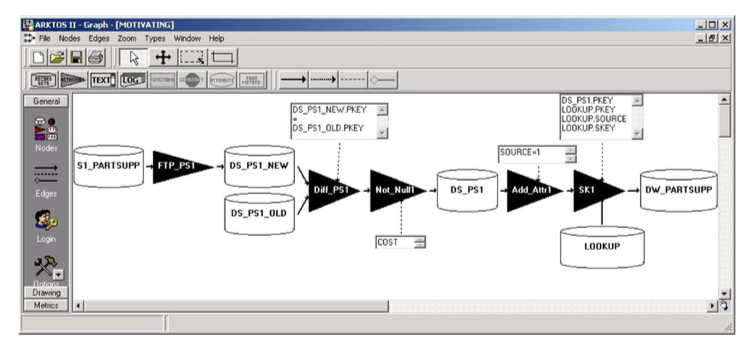
\includegraphics[scale=0.5]{fig/arktosii.png}
	\caption{Exemplo da Ferramenta ARKTOS II em uso (Adaptado de \cite{vassiliadis:2005})}
	\label{arktosii}
\end{figure}

A customização no ARKTOS II é oferecida pela reusabilidade de seus \textit{templates}. Os processos são armazenados em um repositório implementado em um banco de dados relacional. Os autores do ARKTOS II ainda pretendem melhorar a ferramenta permitindo mais formatos de dados como XML e orientado a objetos.


\section{PygramETL}

PygramETL é um \textit{framework} programável para desenvolvedores de ETL. Ele oferece a funcionalidade para desenvolver ETL demonstrando como deve-se iniciar um projeto. O propósito da ferramenta é facilitar a carga dos dados no DW gerenciado por banco de dados relacionais (RDBMS). Focando nos RDBMS como destino torna o desenvolvimento simples, não considerando outros tipos de estrutura de dados e a integração deles. Dessa forma, o PygramETL oferece suporte apenas a bancos de dados relacionais (\cite{thomsen:2009}).

\section{ETLMR}
ETLMR é um framework de ETL que utiliza \textit{MapReduce} para atingir escalabilidade. Ele suporta esquemas de DW como o esquema estrela, o \textit{snowflake}, e o \textit{slowly changing dimensions} \cite{liu:2011}. 

A figura \ref{etlmr} ilustra o fluxo de dados usando o ETLMR usando MapReduce. O processamento da dimensão é feito em uma tarefa do MapReduce, e o processamento do fato é feito por outra tarefa MapReduce. A tarefa MapReduce gera um número de tarefas map/reduce paralelas para processar a dimensão ou o fato. Cada tarefa consiste em inúmeros passos, incluindo a leitura dos dados no sistema de arquivos distribuído (DFS - distributed file system), execução da função de mapeamento, particionamento, combinação do mapeamento de saída, execução da função reduce e escrita dos resultados(\cite{liu:2011}).

\begin{figure}[h]
	\centering
	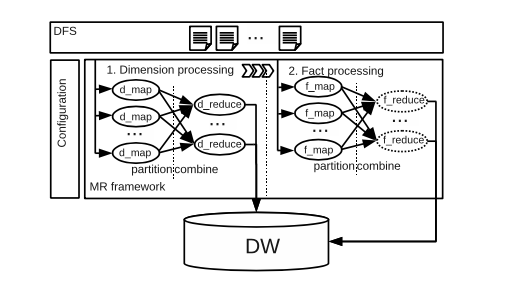
\includegraphics[scale=0.9]{fig/etlmr.png}
	\caption{Fluxo de dados ETL no framework MapReduce (Adaptado de \cite{liu:2011})}
	\label{etlmr}
\end{figure}

O ETLMR possui inúmeras contribuições, ele permite construir dimensões de ETL em alto nível processando os esquemas estrela, snowflake, SCDs e dimensões de dados intensivos. Pelo fato dele utilizar MapReduce, ele pode automaticamente processar mais de um nó enquanto ao mesmo tempo fornece a sincronização dos dados através dos nós. Além da escalabilidade, ele oferece alta tolerância à falhas, possui código aberto, e é fácil de usar com um único arquivo de configuração executando todos os parâmetros.

O principal objetivo do ETLMR é otimizar o tempo de processamento dos processos de ETL por meio do framework MapReduce. Porém, não há nada a respeito de como deve ser feita a modelagem dos processos de ETL.

\section{CloudETL}

O framework CloudETL é uma solução para processos de ETL que usa \textit{Hadoop} para paralelizar fluxos de ETL e \textit{Hive} para processar os dados de forma distribuída. Para o CloudETL o \textit{Hadoop} é a plataforma de execução dos processos de ETL e o \textit{Hive} é o sistema de armazenamento. Conforme a figura \ref{cloudetl}, os componentes do CloudETL são as APIs (interfaces de programação de aplicação), um conjunto de elementos para efetuar as transformações nos dados identificados como ETL \textit{transformers}, e um gerenciador de tarefas que controla a execução das tarefas submetidas ao \textit{Hadoop}. 

CloudETL fornece suporte de alto nível em ETL para construção de diferentes esquemas de DW, como esquema estrela, \textit{snowflake} e SCD (\textit{slowly changing dimensions}). Ele facilita a implementação de processos de ETL em paralelo e aumenta a produtividade do programador significativamente. Esta abordagem facilita as atualizações de SCDs em um ambiente distribuído \cite{liu:2013}.

\begin{figure}[h]
	\centering
	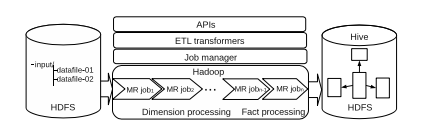
\includegraphics[scale=0.9]{fig/cloudetl.png}
	\caption{Arquitetura do CloudETL (Adaptado de \cite{liu:2013})}
	\label{cloudetl}
\end{figure}

O CloudETL é uma alternativa quando o problema é o processamento de um grande volume de dados por possuir a propriedade de processamento distribuído, porém não oferece nenhum suporte para modelagem de processos de ETL ficando a cargo do programador ou da equipe responsável pelo projeto de DW. 


\section{P-ETL}

P-ETL (Parallel - ETL) foi desenvolvido utilizando o \textit{framework} Hadoop com o paradigma MapReduce. Ele oferece duas maneiras de ser configurado: por meio de uma GUI (\textit{graphical user interface}) ou um arquivo de configuração XML. A figura \ref{petl} mostra a interface gráfica de configuração do P-ETL, ela é organizada em três abas: \textit{Extract, Transform, Load} e uma parte para parâmetros avançados. 

O processo de ETL do \textit{framework} inicia-se na aba \textit{Extract}, as configurações fornecidas pelas outras abas dependem desta primeira, principalmente o formato dos dados da fonte e sua estrutura. O primeiro passo da fase de extração é localizar a fonte de dados.  O arquivo base do P-ETL é no formato "csv" (\textit{Comma Separated Values}). Ele converte a fonte para o formato "csv" permitindo a entrada dos dados em vários formatos. Para acelerar a carga dos dados da fonte no HDFS (formato utilizado pelo \textit{Hadoop}), o P-ETL permite o usuário comprimi-los. A respeito da partição, o usuário pode escolher o tipo de partição (\textit{single, Round Robin, Round Robin by block}) e o número de dados por partição, além disso, ele pode configurar a extração pela quantidade de tuplas (por linhas ou blocos). A aba \textit{Transform} permite o usuário escolher um lista de funções para transformação, cada função deve ser especificamente configurada (condições, expressões, entradas, etc.), assim, as funções são executadas na ordem que foram inseridas. E finalmente, a aba \textit{Loading} permite configurar as tarefas de carga e incluir o destino dos dados (\textit{data warehouse, datamart, etc.}), os dados são comprimidos antes de serem carregados no HDFS e o separados no formato "csv" (\cite{bala:2014}).

\begin{figure}[h]
	\centering
	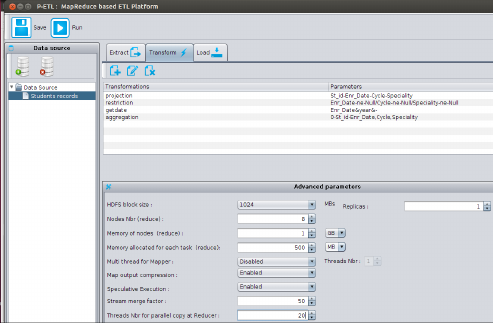
\includegraphics[scale=0.9]{fig/petl.png}
	\caption{Interface de configuração do P-ETL (Adaptado de \cite{bala:2014})}
	\label{petl}
\end{figure}

 O P-ETL usa principalmente dois módulos do \textit{framework} Apache Hadoop: (i) HDFS para o armazenamento distribuído e a alta vazão para o acesso aos dados das aplicações, e (ii) MapReduce para processar paralelamente. Futuramente, o P-ETL pretende adicionar outras funções de transformação para realizar processos mais complexos, e oferecer um ambiente na nuvem, mais precisamente, virtualizar e transformá-lo numa arquitetura orientada à serviço (SOA - \textit{Service Oriented Architecture}) (\cite{bala:2014}).


\section{Big-ETL}

\cite{bala:2015} propõe em seu trabalho uma abordagem chamada Big-ETL, no qual define que funcionalidades de ETL podem ser executadas em \textit{cluster} utilizando o paradigma MapReduce (MR). O Big-ETL permite paralelizar e distribuir o processo de ETL em dois níveis: o processo de ETL (nível de granularidade maior), e a funcionalidade de ETL (nível de granularidade menor); dessa forma, melhorando o desempenho. Para testar a abordagem proposta, o autor utilizou o P-ETL com intuito de melhorar a ferramenta definindo o processo de ETL (nível de granularidade maior), e a funcionalidade de ETL (nível de granularidade menor) como níveis para o experimento, demonstrando ser uma boa alternativa para melhorar o desempenho nos processos de ETL.

Futuramente os autores pretendem apresentar um \textit{benchmark} no qual comparará quatro abordagens: processo de ETL centralizado; processo de ETL distribuído, Big-ETL e uma abordagem híbrida.

\section{FramETL}

O FramETL é um \textit{framework} para desenvolvimento de aplicações ETL. Ele oferece um ambiente programável e integrado para modelagem e execução de processos de ETL utilizando uma linguagem de programação. O autor utilizou conceitos de \textit{frameworks} como flexibilidade, extensibilidade, reuso e inversão de controle para o desenvolvimento do FramETL. Por meio desses conceitos, utilizando o \textit{framework}, o autor pode aplicar sua solução para construções de duas aplicações de ETL. Porém, \cite{silva:2012} não fez uso de BDs NoSQL, e o foco de sua ferramenta não era em dados \textit{Big Data}.

\section{Outras Ferramentas}

Esta seção apresenta outras ferramentas de ETL presentes no mercado e na literatura, mas que não possuem um foco em BDs NoSQL e \textit{Big Data}.
\subsection{Pentaho}

Pentaho Data Integration (conhecido também por \textit{\textbf{Kettle}}) é uma ferramenta \textit{open source} para aplicações de ETL. Ela é composta basicamente por quatro elementos: extração de diferentes fontes, transporte de dados, transformação dos dados e carga no \textit{data warehouse}. O \textit{Kettle} pode ser implementado em um único nó, bem como na nuvem, ou em \textit{cluster}. Ele pode carregar e processar \textit{big data} de várias formas oferecendo flexibilidade e segurança (\cite{mali:2015}, \cite{ETLtools}, \cite{pentaho}). Porém, por ser uma ferramenta genérica ela é de difícil customização. 

\subsection{Talend Studio}

\textit{Talend Open Studio} é uma plataforma de integração de dados que possibilita processos de integração, seu monitoramento e opera como um gerador de código, produzindo \textit{scripts} de transformação. Ele possui um repositório de metadados no qual fornece os dados (definições e configurações relacionados a cada tarefa) para todos os seus componentes. O Talend Studio é comumente utilizado para migração de dados, sincronização ou replicação das bases de dados  (\cite{mali:2015}, \cite{ETLtools}). 

\subsection{CloverETL}

\textit{Clover} é uma ferramenta ETL de código aberto considerada para transformação e integração, limpeza e distribuição de dados em aplicações, banco de dados e \textit{data warehouses}. Ela é baseada em Java e pode ser utilizada em linha de comando e é independente de plataforma  (\cite{mali:2015}).

\subsection{Oracle Data Integrator (ODI)}

\textit{Oracle Data Integrator} é uma plataforma de integração de dados que atende diversos requisitos de integração, desde grandes volumes de dados até o carregamento em \textit{batch}. As bases de dados de origem e destino podem incluir base de dados relacionais, arquivos XML, tabelas \textit{Hive, Hbase}, arquivos \textit{HDFS}, entre outros. Os usuários podem inserir filtros, junções, agregações, e outros componentes de transformação (\cite{silva:2016}). Porém, o ODI é uma ferramenta comercial e não permite a customização de suas aplicações.

\section{Considerações Finais}

Este capítulo discorreu a respeito das ferramentas de ETL encontradas na literatura. A maioria foca no desempenho ao lidar com \textit{Big Data}, nenhuma delas apresentou uma solução alternativa para modelagem de BDs NoSQL ficando a cargo do desenvolvedor encontrar meios para esquematizar os dados. A ferramenta P-ETL (\cite{bala:2014}) apresentou um arquivo "csv" como alternativa para obter diversos tipos de dados, porém não há um enfoque em BDs NoSQL. A abordagem PygramETL (\cite{thomsen:2009}) facilita a carga de dados, mas lida apenas com banco de dados relacionais. Para suportar processos de ETL em BDsNoSQL, propomos um \textit{framework} integrado, flexível e programável de ETL para BDs NoSQL que permite o uso do processamento distribuído/paralelo e a integração das diversas bases de dados existentes por se tratar de um \textit{framework} baseado em componentes.  